\chapter{Relation with Wizard of Oz}\label{chap:woz}
\begin{framed}
	\textbf{Key points:}
	
	\begin{itemize}
		\item An experiment was designed to explore the influence of \gls{sparc} on the human workload and task performance compared to an approach based on \gls{woz}.
		\item Application target replaced by a robot to ensure repeatability of target behaviour.
		\item Design of a robot model exhibiting probabilistic behaviour with a non-trivial optimal interaction policy.
		\item Results show that \gls{sparc} achieves a similar performance than \gls{woz} while requiring a lower workload from the teacher.
	\end{itemize}
\end{framed}

Parts of the work presented in this chapter have been published in \cite{senft2015sparc} \footnote{Note about technical contribution in this chapter: the author used software from the \gls{dream} project for the touchscreen and the robot functionalities. The author contributed to the material used within the robot control and the Graphical User Interface. Algorithm used from the OPENCV neural network library.} . The final publication is available from Springer via \url{http://dx.doi.org/10.1007/978-3-319-25554-5_60}.

\newpage

\section{Motivation}

SPARC as been designed to enable end-users non-experts in computer science to teach a robot an action policy while interacting in a sensitive environment. The argument behind this way of interacting is that SPARC allows a field expert to transfer their knowledge to an autonomous agent without wasting time to teach the agent and having to enforce each actions manually. As the agent is interacting in the target environment, displaying a appropriate action policy, the time spend to teach it is not lost as the desired interaction takes place also during the learning phase. For example, using the context of \gls{rat}, the therapist would teach the robot during a therapy session. As the therapist is in total control of the robot's action, the behaviour expressed by the robot fits the desired behaviour desired for the therapy.

In essence, SPARC, as a principle, allows to start a robotic application in a \gls{woz} fashion, and then move away from it as the robot gains autonomy. The aim of SPARC is two fold: maintaining a high level of performance while reducing the workload of the teacher over time until reaching a point where the robot is autonomous or only necessitate minimal supervision to interact successfully. As explained in Chapter \ref{chap:sparc}, SPARC involves two interactions the control interaction and the application ones. And when the goal is learning how to interact with humans, the robot is interacting simultaneously with two humans. These two dependent interactions complexify the evaluation of the approach, especially as both humans are impacting each other. The first step to evaluate SPARC was to focus on the relation between the robot and its teacher. To evaluate this aspect of the interaction, we decided to replace the target of the application by a robot running a model of a child and observe the impact of SPARC on the teacher. The setup ends up with two robots interacting together (the wizarded-robot and the child-robot) whilst the wizarded-robot is controlled by a participant. The child-robot has some inner variables (motivation and engagement) and has to keep them high to achieve a good performance.

\section{Hypotheses}

To evaluate the validity of SPARC and the influence of such an approach, four hypotheses were devised:
\begin{enumerate}
	\item [H1] A `good' teacher (i.e. keeping the motivation and engagement of the child-robot high) will lead to a better child-robot performance.
	\item [H2] When interacting with a new system, humans will progressively build a personal strategy that they will use in subsequent interactions.
	\item [H3] Reducing the number of interventions required from a teacher will reduce their perceived workload.
	\item [H4] Using SPARC allows the teacher to achieve similar performance with fewer interventions than \gls{woz}.
\end{enumerate}

H1 represents a sanity check for the model, ensuring that the expressed performance represents the efficiency of the action policy demonstrated by the teacher. H2 tests that human teachers are not static entities, they adapt their learning target and their teaching strategy. H3 tests one of the motivations behind SPARC: does reducing the number of physical actions required for a robot to interact while requiring the teacher to monitor the robot suggestions lead to a lower workload. And finally, H4 is the main hypothesis, does SPARC enable a robot to learn a useful action policy: reducing the teacher's workload while maintaining a high performance.

\section{Methodology}

This study is based on a real scenario for \gls{rat} for children with \gls{asd} based on the Applied Behaviour Analysis therapy framework. The aim of the therapy is to help the child to develop/practice their social skills. The child has to complete an emotion recognition task involving a child playing a categorisation game with a robot on a mediating touchscreen device \cite{baxter2012touchscreen}. And the robot can provide feedback and prompts to encourage the child and help them to classify emotions. Images of faces or drawings are shown to the child, and they have to categorise them by moving the image to one side or the other depending on whether the picture shown denotes happiness or sadness (e.g. fig. \ref{fig:setup}). In the therapy, the robot is remote controlled by an operator using the \acrlong{woz} paradigm, and does not interact with the child directly. 

This study explores if \gls{sparc} can be used to teach the robot a correct action policy to interact with the child. As timing in human-robot interactions is complex, for simplification reasons, the interaction has been discretised to have clear steps when the robot has to select an action. The basic interaction structure following SPARC is as follows: 
\begin{enumerate}
	\item the robot suggests an action to the teacher
	\item the teacher can select an action for the robot to execute or let the proposed action be executed
	\item the robot executes the selected action 
	\item both robot and teacher observe the outcome of the action until the next action selection step
\end{enumerate}

Using \gls{sparc}, over time, the robot learns to replicate the teacher's policy by matching the inputs (child's state) to the outputs (action selected by the teacher). 

%the policy used by the teacher based on observations of the child and the oversight from the teacher, with the teacher still maintaining overall control if necessary.

Two conditions are compared: SPARC, where the robot learns from the human corrections and the \gls{woz} condition, where the robot proposes a random actions instead of learnt actions to simulate a \gls{woz} setup where the teacher would have to select every the actions.

The focus of the study being on the \textit{control interaction} (the relation between the teacher and the robot), the second interaction (the application one) has been kept constant by replacing the child by a robot. A minimal model of child behaviour is therefore used to stand in for a real child. A second robot is employed in the interaction to embody this child model: we term this robot the \textit{child-robot} while the robot being directly guided by the human teacher is the \textit{wizarded-robot} (Figure \ref{fig:woz_setup}).

\begin{figure}[t!]
	\centering
	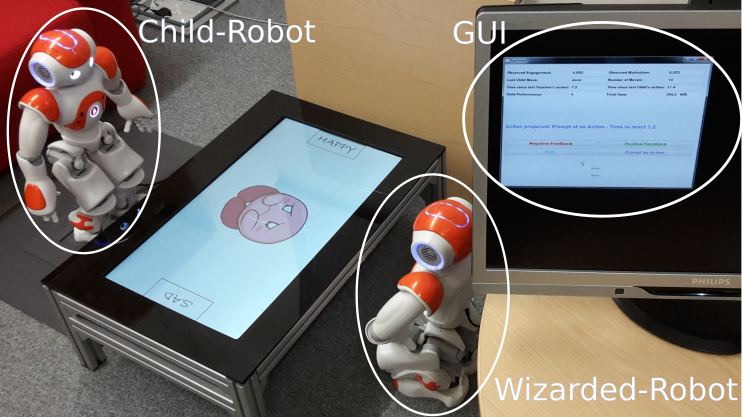
\includegraphics[width=0.65\textwidth]{woz_setup_annotated.png}
	\caption{Setup used for the user study from the perspective of the human teacher. The \textit{child-robot} (left) stands across the touchscreen (centre-left) from the \textit{wizarded-robot} (centre-right). The teacher can oversee the actions of the \textit{wizarded-robot} through the \gls{gui} and intervene if necessary (right).}
	\label{fig:woz_setup}
\end{figure}
		
\subsection{Child model} \label{ssec:woz_child}

The purpose of the child model is not to realistically model a child (with or without autism), but to provide a means of expressing some characteristics of the behaviours we observed in interactions with children in a repeatable manner. The child-robot possesses an internal model encompassing an \emph{engagement} level and a \emph{motivation} level, together forming the \textit{state} of the child. The engagement represents how often the child-robot will make categorisation moves and the motivation gives the probability of success of the categorisation moves. Bound to the range $[-1, 1]$, these states are influenced by the behaviour of the wizarded-robot, and will asymptotically decay to zero without any actions from the wizarded-robot. These two states are not directly accessed by either the teacher or the wizarded-robot, but can be observed through behaviour expressed by the child-robot: low engagement will make the robot look away from the touchscreen, and the speed of the categorisation moves is related to the motivation (to which gaussian noise was added). There is thus incomplete/unreliable information available to both the wizarded-robot and the teacher, making the task non-trivial.

The influence of the wizarded-robot behaviour on the levels of engagement and motivation are described below (Section \ref{ssec:woz_wizarded_robot}). In addition to this, if a state is already high and an action from the wizarded-robot should increase it further, then there is a chance that this level will sharply decrease, as an analogue of \textit{frustration}. When this happens, the child-robot will indicate this frustration verbally (uttering one of eight predefined strings). This mechanism prevent the optimal strategy to be straightforward: always making actions aiming to increase motivation or engagement. The optimal strategy includes these actions but also waiting times to prevent the state values to overshoot. This non-trivial optimal strategy approximates better a real human-robot interaction scenario requiring a more complex strategy to be employed by the teacher.

\subsection{Wizarded-robot control}
\label{ssec:woz_wizarded_robot}
The wizarded-robot is controlled through a \gls{gui} and has access to multiple variables characterising the state of the interaction as used by the learning algorithm:
\begin{itemize}
	\item Observed engagement
	\item Observed motivation
	\item Type of last move made by the child-robot (good/bad/done)
\end{itemize}
Additionally, other metrics are displayed to the teacher but not used in the algorithm:
\begin{itemize}
	\item Number of categorisations made by the child-robot
	\item Time since last teacher's action
	\item Time since last child's action
	\item Child's performance
	\item Total time elapsed
\end{itemize}


The wizarded-robot has a set of four actions, with one button each on the \gls{gui}: 
\begin{itemize}
	\item Prompt an Action: Encourage the child-robot to do an action.
	\item Positive Feedback: Congratulate the child-robot on making a good classification.
	\item Negative Feedback: Supportive feedback for an incorrect classification.
	\item Wait: Do nothing for this action opportunity, wait for the next one.
\end{itemize}

The impact of actions on the child-robot depends on the internal state and the type of the last child-robot move: good, bad, or done (meaning that feedback has already been given for the last move and supplementary feedback is not necessary). A \textit{prompt} increases the engagement, a \textit{wait} has no effect on the child-robot's state, and the impact of positive and negative feedback depends on the previous child-robot move. Congruous feedback (positive feedback for correct moves; negative feedback for incorrect moves) results in an increase in motivation, but incongruous feedback can decrease both the motivation and the engagement of the child-robot. The teacher therefore has to use congruous feedback and prompts.

However, as mentioned in Section \ref{ssec:woz_child}, if engagement or motivation cross a threshold, their value can decrease abruptly to simulate the child-robot being frustrated. This implies that the optimal actions policy provides congruous feedback and prompts, but also requires wait actions to prevent the child-robot becoming frustrated and keep its state-values close to the threshold without crossing it. A `good' strategy keeping the engagement and motivation high, leads to an increase in performance of the child-robot in the categorisation task.

To simplify the algorithm part, the interaction has been discretised: the teacher can not selects actions for the wizarded-robot at any time, actions can only be executed at specific times triggered by the wizarded-robot: two seconds after each child-robot action, or if nothing happens in the interaction for five seconds. When these selection windows are hit, the wizarded-robot proposes an action to the teacher by displaying the action's name and a countdown before execution. Only after this proposition has been done can the teacher select a different action for the wizarded-robot or let the proposed one be executed: if the teacher does nothing in the three seconds following the suggestion, the action proposed by the wizarded-robot is executed. This mechanism allows the teacher to passively accept a suggestion or actively make an \emph{intervention} by selecting a different action and forcing the wizarded-robot to execute it.

\subsection{Learning algorithm}

In the SPARC condition, the robot learns to reproduce the action policy displayed by the teacher. For this study, the robot learns using a Multi-Layer Perceptron (MLP): with five input nodes: one for the observed motivation, one for the observed engagement and three binary (+1/-1) inputs for the type of the previous move: good, bad, or done. The hidden layer had six nodes and the output layer four: one for each action. The suggested action is selected applying a Winner-Take-All strategy on the value of the output node and then displayed on the \gls{gui} before execution. The network is trained with back propagation: after each new decision from the teacher a new training point is added with the selected action node having +1 while the others -1. The network is fully retrained with all the previous state-action pairs and the new one at each selection step. 
%The network was using sigmoid activation function and a learning rate of 0.6 (probably).

This learning algorithm, MLP is not optimal for a real time interaction as the online learning should happens quickly between learning iteration. However as the length of interaction (and so the number of datapoints) is limited and the desired learning behaviour is purely supervised learning, this type of algorithm has been deemed suitable for this study.
%On the other side, the random controller proposed random actions to the teacher.

\subsection{Participants}

In \gls{rat} scenarios using \gls{woz} to control the robot, the wizard is typically a technically competent person with previous experience controlling robots or at least significant training controlling this robot for the therapy. As such, to maintain consistency with the target user group, the participants of this study (assuming the role of the teacher) have been taken from a robotics research group. Ten participants were used (7M/3F, age \textit{M}=29.3, 21 to 44, \textit{SD}=4.8 years).

\subsection{Interaction Protocol}

The study compared two conditions: a learning robot adapting its propositions to its user (the \gls{sparc} condition) and a non-learning robot constantly proposing random actions (the \gls{woz} condition). The child-robot controller was kept constant in both conditions, while the state is reset between interactions. The design was a within subjects comparison with balancing of order: each participant interacted with both conditions, with the order balanced between participants to control for any ordering effects. In \textit{order LN} the participants first interact with the learning wizarded-robot in the \gls{sparc} condition, and then with the non-learning one in the \gls{woz} condition; in \textit{order NL} the order of interaction is inverted. Participants were randomly assigned to one of the two orders.

The interactions took place on a university campus in a dedicated experiment room. Both robots were Aldebaran Nao, one of which had a label indicating that it was the \emph{Child-Robot}. The robots faced each other with a touchscreen between them, and participants assuming the role of the teacher sat at a desk to the side of the wizarded-robot, with a screen and a mouse to interact with the wizarded-robot (fig. \ref{fig:woz_setup}). Participants were able to see the screen and the child-robot.

%ADD ref annex
A document explaining the interaction scenario was provided to participants with a demographic questionnaire (cf Annexes. ). After the information had been read, a 30s video presenting the \gls{gui} in use was shown to familiarise the participants with it, without biasing them towards any particular control strategy. Then participants clicked a button to start the first interaction which lasted for 10 minutes. The experimenter was sat in the room outside of the participants' field of view. After the end of the first interaction, a post-interaction questionnaire was administered. The same protocol was applied in the second part of the experiment with another post-interaction questionnaire following. Finally, a post-experiment questionnaire asking participants to explicitly compare the two conditions was administered.

\subsection{Measures}

Two types of measures have been recorded for this study: interaction data representing objective behaviours and performance of the participants and subjective data through questionnaires.

\paragraph{Interaction data}

The state of the child-robot and the interaction values were logged at each step of the interaction (at 5Hz). All of the human actions were recorded: acceptance of the wizarded-robot's suggestion, selection of another action (intervention), and the states of the child-robot (motivation, engagement and performance) at this step. 

The first metric is the performance achieved in each interaction measured by the number of correct categorisations made by the child-robot minus the number of incorrect ones. This represents how correct was the action policy executed by the wizarded-robot when controlled by a participant.

The second important metric is the intervention ratio: the number of times a user chooses a different action than the one proposed by the wizarded-robot, divided by the total number of executed actions. This metric represents how often in average a user had to correct the robot and could be related to the workload the user had to face to control the robot.

\paragraph{Questionnaire data}
 
Participants answered to four questionnaires: a demographic one, before the interaction, two post-interaction ones where they were asked to evaluate the last interaction with the robots and a post-experiment where they had to compare the two conditions and select the one corresponding to a description. All the rating questionnaires used seven items Likert scale.

\paragraph{Post-Interaction}
\begin{itemize}
	\item The child-robot learned during the interaction
	\item The performance of the child-robot improved in response to the teacher-robot actions
	\item The teacher-robot is capable of making appropriate action decisions in future interactions without supervision
	\item The teacher-robot always suggested an incorrect or inappropriate actions
	\item By the end of the interaction, my workload was very light
	\item What did you pay most attention during the interaction? (child-robot, touchscreen, \gls{gui}, other)
\end{itemize}

\paragraph{Post-experiment}
\begin{itemize}
	\item There was a clear difference in behaviour between the two teacher-robots
	\item There was a clear difference in behaviour between the two child-robots
	\item Which teacher-robot was better able to perform the task? (first, second)
	\item Which teacher-robot did you prefer supervising? (first, second)
\end{itemize}

\section{Results}

\subsection{Interaction data}

Figure \ref{fig:woz_comp} presents the aggregated (results collapsed between orders) performance and intervention ratio for both conditions. While the number of participants are not sufficient to perform statistical comparison, overall interaction results seem to show that both conditions lead to similar performance (\gls{sparc}: 32.6 (95\% CI [27.89,37.31]) - \gls{woz}: 31.4 (95\% CI [25.9,36.9])) while the \gls{sparc} condition required less intervention (\gls{sparc}: 0.38 (95\% CI [0.29,0.47]) - \gls{woz}: 0.59 (95\% CI [0.52,0.67])). 

\begin{figure*}[ht]
	\centering
	\begin{subfigure}[t]{0.5\textwidth}
		\centering
		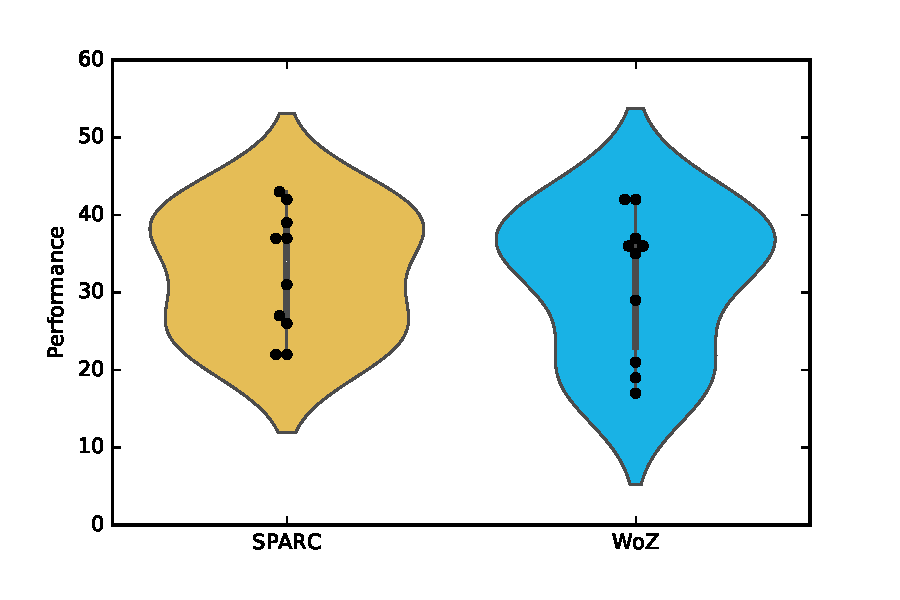
\includegraphics[width=1.0\textwidth]{./images/woz_perf.pdf}
%		\caption{Comparison of end performance for both conditions.}
	\end{subfigure}%
	~ 
	\begin{subfigure}[t]{0.5\textwidth}
		\centering
		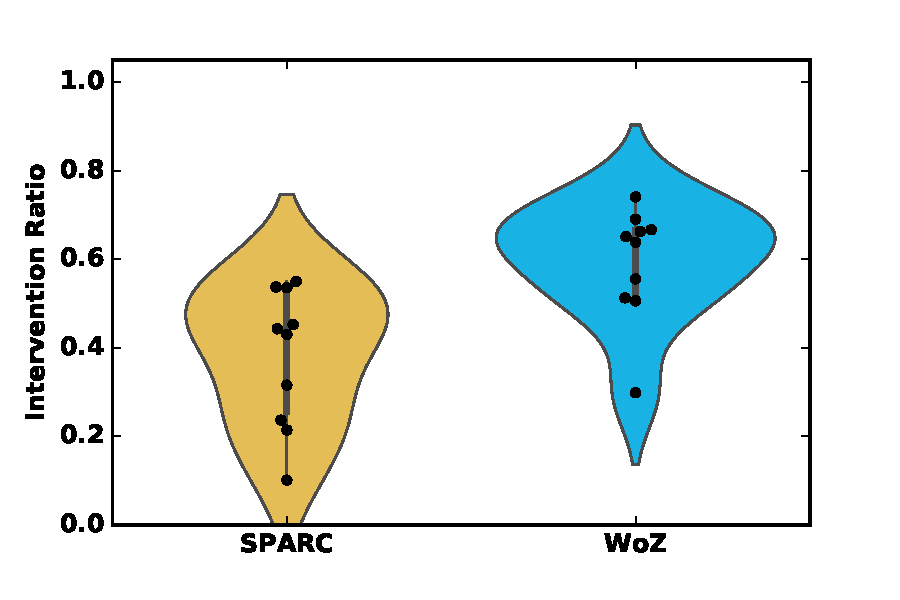
\includegraphics[width=1.0\textwidth]{./images/woz_ratio.pdf}
%		\caption{Comparison of intervention ratio for both conditions.}
	\end{subfigure}
	\caption{Aggregated comparison of performance and intervention ratio for both conditions}
	\label{fig:woz_comp}
\end{figure*}

Figure \ref{fig:woz_ratio_time} presents the evolution of intervention ratio for each condition and orders. During the first interaction, participants discover the interface and how to interact with it, which results in a high variation intervention ratio in the first 20 steps (each time the wizarded-robot proposes an action). However in the second phase of the interaction,  when participants develop their teaching policy, there is a tendency of \gls{sparc} requiring a lower number of intervention than \gls{woz}. This effect is higher in the second interaction, where as soon as 5 steps, the two conditions differentiate without overlap of the 95\% CI of the mean, which would indicate that the two conditions differ in term of required interventions.

\begin{figure}[ht]
	\centering
	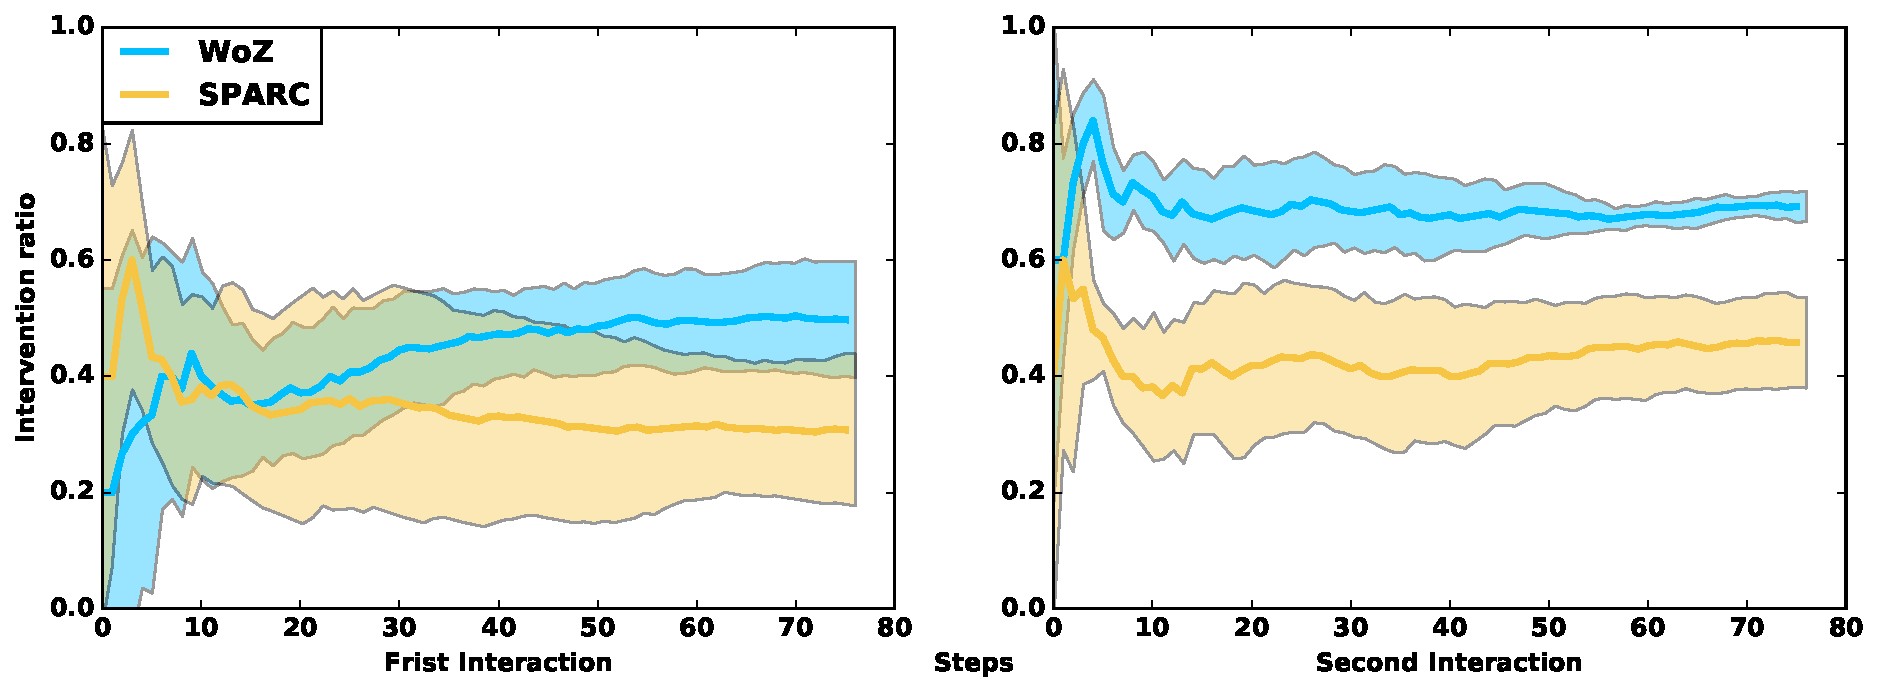
\includegraphics[width=1.\textwidth]{./images/woz_ratio_time.pdf}
	\caption{Evolution of intervention ratio over time for both conditions and both orders. Shaded area represents the 95\% CI.}
	\label{fig:woz_ratio_time}
\end{figure}

Both for the performance and the intervention ratio, a strong ordering effect have been observed. Figure \ref{fig:woz_separated} and Table \ref{tab:woz_comp_means} present the performance and intervention ratio separated by condition and order. In both orders, the second interaction had higher performance as the participants were used to the system and understood how to develop an efficient interaction policy. And the performance between condition is similar. However, regardless of the order, when only the interaction number is considered, the intervention ratio is lower when using \gls{sparc} compared to \gls{woz}. This indicates that when the wizarded-robot learned using \gls{sparc}, a similar performance is attained as with \gls{woz}, but the number of interventions required to achieve this performance is lower.

%COuld use the CIDM if desired or not

\begin{figure}[ht]
	\centering
	\begin{subfigure}[t]{0.5\textwidth}
		\centering
		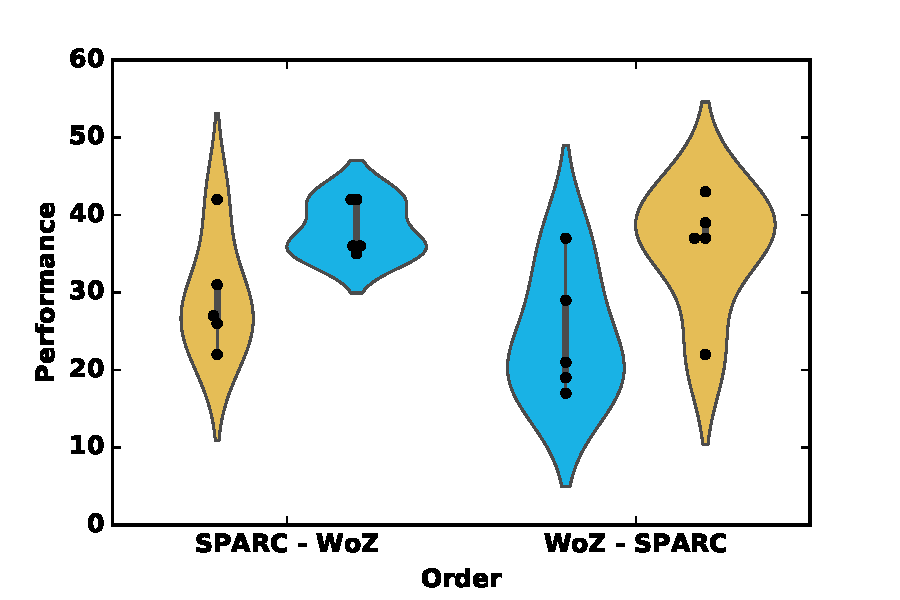
\includegraphics[width=1.\textwidth]{./images/woz_perf_divided.pdf}
	\end{subfigure}%
	~ 
	\begin{subfigure}[t]{0.5\textwidth}
		\centering
		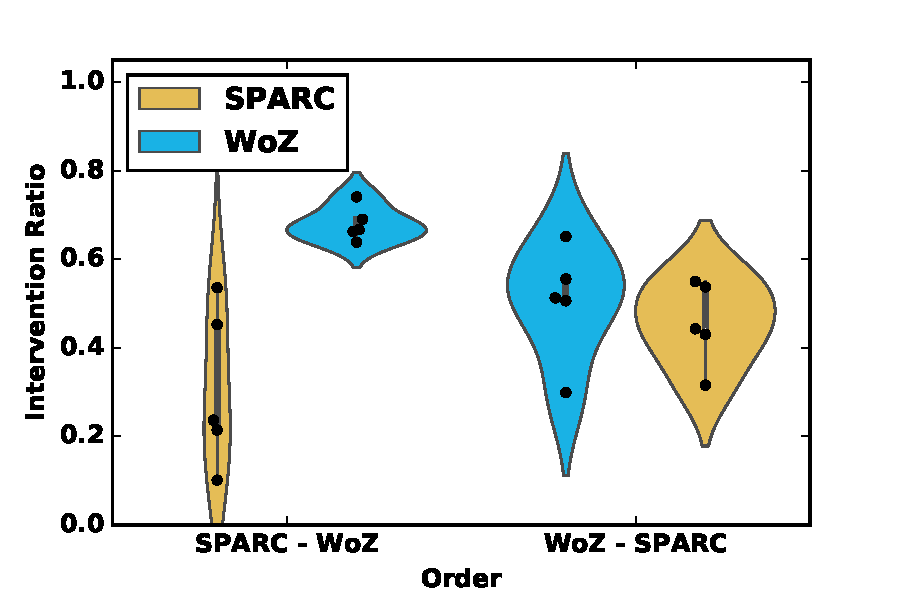
\includegraphics[width=1.\textwidth]{./images/woz_ratio_divided.pdf}
	\end{subfigure}
	\caption{Performance achieved and intervention ratio separated by order and condition. For each order, the left part presents the performance in the first interaction (with one condition) and the right part the performance in the second interaction (with the other condition).}
	\label{fig:woz_separated}
\end{figure}


\begin{table}[t]
	\caption{Average performance and intervention ratio separated by condition and order.}
	\centering
\begin{tabulary}{1.0\textwidth}{L"C"C"C|C}
	& \multicolumn{2}{c"}{Order LN} & \multicolumn{2}{c}{Order NL} \\
	& SPARC (int 1) & WoZ (int 2) & WoZ (int 1) & SPARC (int 2) \\
	\hline			
Performance M \linebreak 95\% CI & 29.6 [23.61,35.59] & 38.2 [35.46,40.94] & 24.6 [18.1,31.1] & 35.6 [29.34,41.86]\\
Intervention Ratio M 95\% CI & 0.31 [0.17,0.45] & 0.68 [0.65,0.71] & 0.5 [0.4,0.61] & 0.46 [0.38,0.53]\\
\end{tabulary}
\label{tab:woz_comp_means}
\end{table}



%In both conditions, the average performance in the second interaction (\textit{M$_{LN-2}$} =38, 95\% CI [36.2, 39.8], \textit{M$_{NL-2}$}=34.8, 95\% CI [30.8, 38.8]) was higher than in the first one (\textit{M$_{LN-1}$}=29.4, 95\% CI [25.3, 33.5], \textit{M$_{NL-1}$}=24.3, 95\% CI [19.4, 29.4]; Fig. \ref{fig:graphs} \textit{left}). The 95\% \textit{Confidence Interval of the Difference of the Mean} (CIDM) for the L-NL condition is [4.1, 13.1] and for the NL-L condition is [4.0, 16.8].
%However, the performance is similar when only the interaction order (first or second) is considered. 
%The participants performed slightly better in the LN condition, but the CIDM includes zero in both cases (95\% CIDM$_{1}$ [-1.5, 11.5], 95\% CIDM$_{2}$ [-1.2, 7.6]). 
%In the condition L-NL, the intervention ratio increased between the learning and non learning condition (\textit{M$_{LN-1}$}=0.31, 95\% CI [0.20, 0.42] to \textit{M$_{LN-2}$}=0.68, 95\% CI [0.66, 0.70], CIDM$_{LN}$=[0.26, 0.48]). 
%But in the NL condition, the intervention ratio is almost identical between the two interactions but slightly lower for the learning case (\textit{M$_{NL-1}$}=0.50, 95\% CI [0.44, 0.57] to \textit{M$_{NL-2}$}=0.46, 95\% CI [0.40, 0.51], CIDM$_{NL}$ [-0.03, 0.13]).

Additionally, a strong positive correlation (Pearson's \textit{r}=0.79) was found between the average child-robot motivation and engagement and its performance which shows that the performance achieved by the child-robot represents the capacity of the teacher to keep both engagement and motivation high.

\subsection{Questionnaire data}

The post-interaction questionnaires evaluated the participant's perception of the child-robot's learning and performance, the quality of suggestions made by the wizarded-robot, and the experienced workload. All responses used seven point Likert scales.

Table \ref{tab:woz_quest_means} presents separated results for the questions asked in the post-interaction questionnaires, with more details for the questions exhibiting differences in Figure \ref{woz_quest}.

Across the four possible interactions, the rating of the child-robot's learning was similar (\textit{M}=5.25, 95\% CI [4.8, 5.7]). As the child-robot was using the same interaction model in all four conditions, this result is expected. There is a slight tendency to rate the child's performance as being higher but the error margin is too high to conclude anything. This could indicate that the teachers were more aware of the child's behaviour as the workload was lighter to control the wizarded-robot.

\begin{table}[t]
	\caption{Average reporting on questionnaires separated by condition and order.}
	\centering
	\begin{tabulary}{1.0\textwidth}{L"C|C"C|C}
		& \multicolumn{2}{c"}{Order LN} & \multicolumn{2}{c}{Order NL} \\
		& SPARC (int 1) & WoZ \linebreak (int 2) & WoZ \linebreak (int 1) & SPARC (int 2) \\
		\hline			
		Child learns M \linebreak 95\% CI & 5.2 [3.69,6.71] & 5.2 [3.8,6.6] & 5.2 [4.18,6.22] & 5.4 [4.7,6.1]\\
		Child's performance M \linebreak 95\% CI & 4.6 [3.41,5.79] & 5.0 [3.25,6.75] & 5.0 [4.04,5.96] & 4.4 [3.7,5.1]\\
		Wizarded-robot makes errors \linebreak M 95\% CI & 1.6 [0.9,2.3] & 4.0 [2.76,5.24] & 2.6 [1.9,3.3] & 2.0 [2.0,2.0]\\
		Wizarded-robot makes appropriate decisions M 95\% CI & 4.8 [3.4,6.2] & 3.6 [2.18,5.02] & 3.0 [2.04,3.96] & 5.2 [4.85,5.55]\\
		Lightness of workload M \linebreak 95\% CI & 4.6 [3.41,5.79] & 3.6 [1.8,5.4] & 3.8 [2.94,4.66] & 5.4 [4.35,6.45]\\
	\end{tabulary}
	\label{tab:woz_quest_means}
\end{table}


Participants rated the wizarded-robot as more suited to operate unsupervised in the learning than in the non learning condition (confidence interval of the difference of the mean (CIDM) for LN ordering [-0.2, 2.6], CIDM for the NL ordering [1.6, 2.8]).

Similarly, a trend was found showing that learning wizarded-robot is perceived as making fewer errors than the non-learning robot (CIDM for LN ordering [1.3, 3.4], CIDM for the NL ordering [0.1, 1.1]). 

The participants tended to rate the workload as lighter when interacting with the learning robot, and this effect is much more prominent when the participants interacted with the non-learning robot first (CIDM for LN ordering [-0.6, 2.6], CIDM for the NL ordering [0.7, 2.5]).

Most of the difference of mean interval exclude 0 or include it marginally, which would indicate tendency of difference (due to the low number of participants, no statistical tests are applicable).

\begin{figure}[ht]
	\centering
	\begin{subfigure}[t]{0.3295\textwidth}
		\centering
		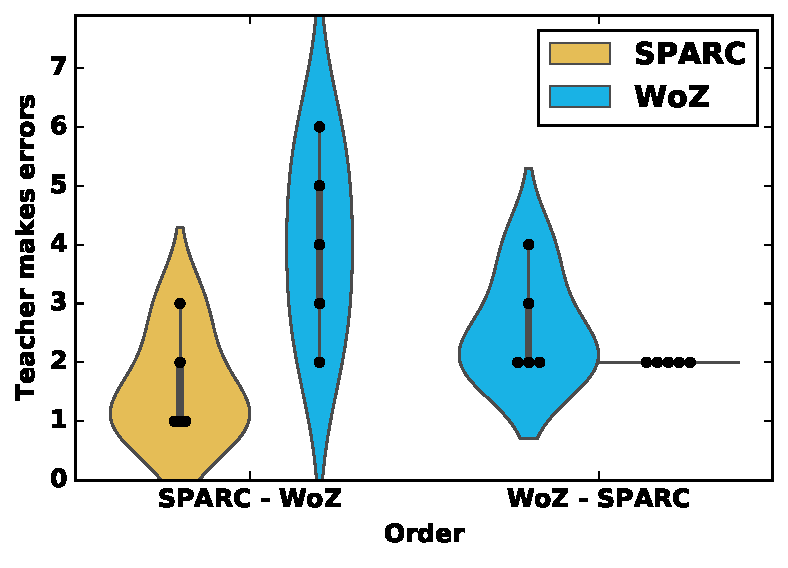
\includegraphics[width=1.\textwidth]{./images/woz_errors.pdf}
	\end{subfigure}%
	~ 
	\begin{subfigure}[t]{0.341\textwidth}
		\centering
		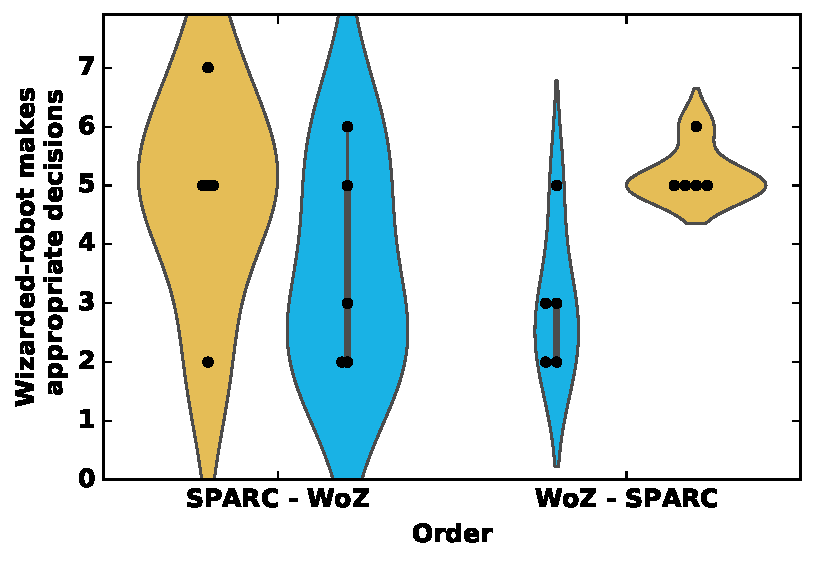
\includegraphics[width=1.\textwidth]{./images/woz_appropriate.pdf}
	\end{subfigure}%
	~ 
	\begin{subfigure}[t]{0.3295\textwidth}
		\centering
		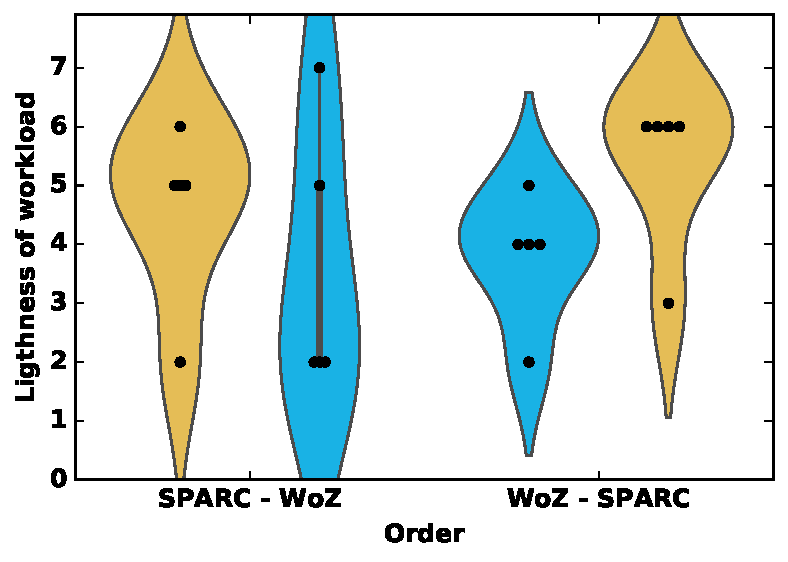
\includegraphics[width=1.\textwidth]{./images/woz_workload.pdf}
	\end{subfigure}
	\caption{Questionnaires results on robot making errors, making appropriate decisions and on lightness of workload.}
	\label{fig:woz_quest}
\end{figure}

\section{Discussion}

\section{Summary}

